\begin{exercise}{Verengtes Rohr}{10}
  Ein Zylinderförmiges Rohr mit einem Durchmesser von $R_{1}=50$ mm ist auf
  einem Zwischenstück verengt und besitzt dort nur noch einen Radius von
  $R_{2}=25$ mm. An der verengten Stelle ist von unten ein weiteres Rohr mit
  einem Radius von $R_{3}=10$ mm angeschlossen, dessen Ende sich in einem
  Wasserbecken befindet. Durch das Rohr flie\ss en 6 L Wasser pro Sekunde.

  \begin{enumerate}
    \item [a)] Welcher Unterdruck entsteht an der verengten Stelle?
    \item [b)] Kann durch das senkrechte Rohr das untere Wasser 1 m hoch gezogen
    werden?
  \end{enumerate}
\end{exercise}

\FloatBarrier

  \begin{figure}[h]
    \centering
    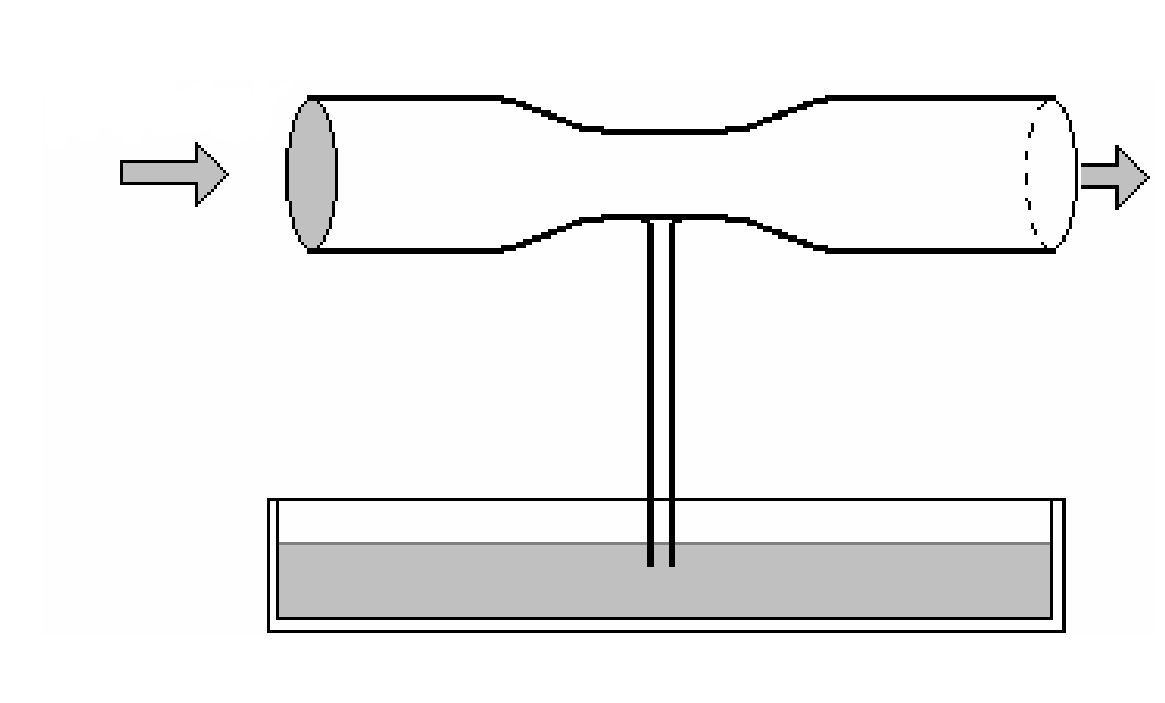
\includegraphics[width = 0.5\textwidth]{Rohr.jpg}
  \end{figure}

\begin{exercise}{Hydrodynamik}{10}
  Ein zylinderförmiger Stab mit Radius $R_1$ bewegt sich mit der Geschwindigkeit $u$
  parallel zu seiner Achse in einem zu ihm koaxialen zylinderförmigen Rohr mit Radius
  $R_2$. Der Raum zwischen dem Stab und dem Rohr ist mit einer inkompressiblen
  Flüssigkeit gefüllt. Die Strömung ist stationär.\\
  Wählen Sie an das Problem angepasste Zylinderkoordinaten $(r, \theta, z)$. Sie
  können davon ausgehen, dass die Geschwindigkeit $\vec{v}$ der Flüssigkeit nur von
  dem radialen Abstand von der Symmetrieachse abhängt und immer in $z$-Richtung zeigt.

  \begin{enumerate}
    \item Welche Gleichung für $v_z$ erhalten Sie ausgehend von der Navier-Stokes-Gleichung?
    \item Welche Randbedingungen gelten? D.h. geben Sie $v_z(r = R_1)$ und $v_z(r = R_2)$ an.
    \item Lösen Sie die Navier-Stokes-Gleichung für diesen Fall. D.h. berechnen Sie $v_z(r)$.
  \end{enumerate}

  \begin{figure}[h]
    \centering
    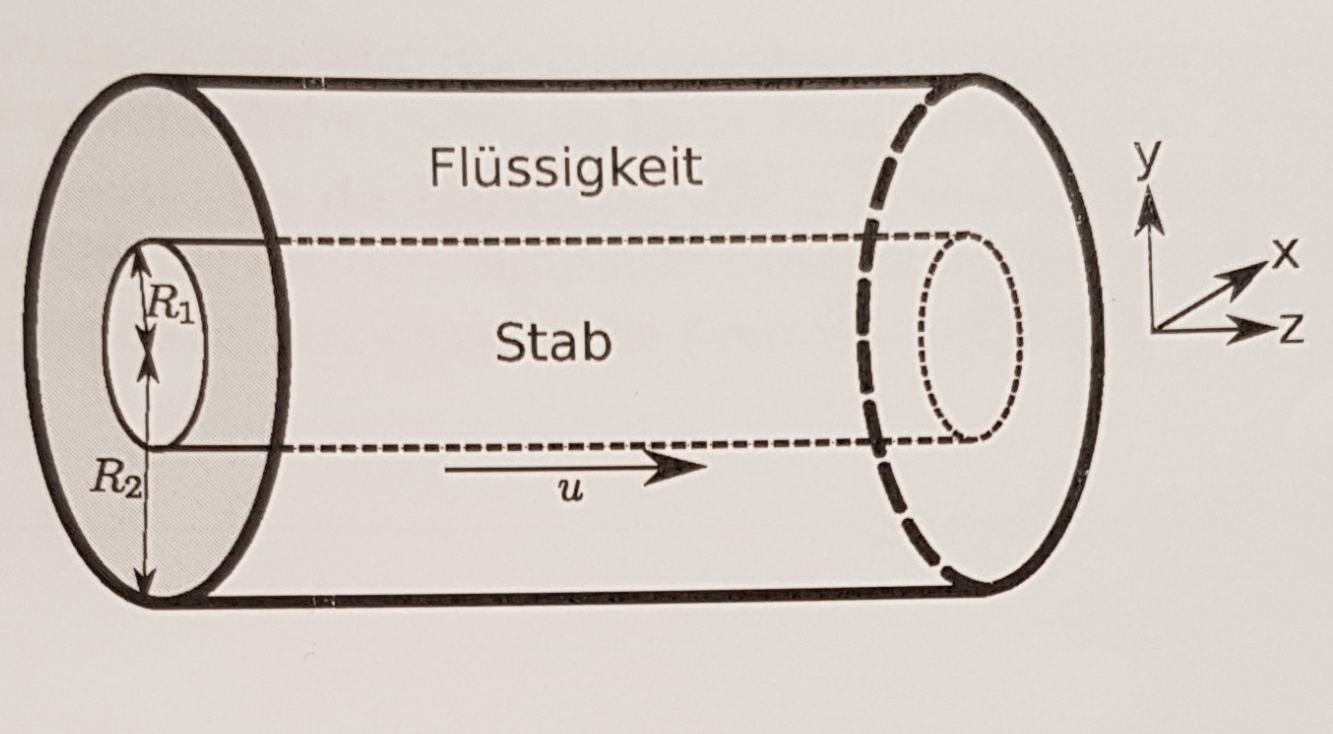
\includegraphics[width=0.8\textwidth]{Skizze_Navier_Stokes.jpg}
    \label{fig:Skizze_Koaxial}
  \end{figure}

\end{exercise}


\FloatBarrier
\newpage

\begin{exercise}{Zusatzaufgabe}{+10}
  \begin{enumerate}
    \item [a)] Bestimmen Sie das elektrische Feld eines unendlich langen Drahtes.
    \item [b)] Bestimmen Sie das magnetische Feld eines unendlich langen Drahtes
               mit dem Durchmesser $R_{0}$. Betrachten Sie dabei auch das Feld
               innerhalb des Leiters.
    \item [c)] Bestimmen Sie das magnetische Feld einer Torroidspule mit innerem
               Radius $r_{1}$ und äu\ss erem Radius $r_{2}$. Betrachten Sie dabei
               alle Bereiche (r<$r_{1}$,$r_{1}$<r<$r_{2}$,r>$r_{2}$).
  \end{enumerate}
\end{exercise}
